\documentclass[a4paper, 12pt]{article}

\usepackage[margin=2cm, top=2.5cm, bottom=2.5cm]{geometry}
\usepackage[ngerman]{babel}
\usepackage[utf8]{inputenc}
\usepackage[T1]{fontenc}
\usepackage[bookmarks]{hyperref}
\usepackage{graphicx}
\usepackage{tabularx}
\usepackage{verbatim}
\usepackage{listings}
\usepackage{color}
\usepackage{expdlist}
\usepackage{etoolbox}

\newenvironment{componenttable}{%
  \par\description\item%
    \tabularx{\linewidth}{>{\ttfamily}l >{\ttfamily}l X}
      \normalfont Name & \normalfont Typ & \normalfont Beschreibung \\%
      \hline%
}{%
    \endtabularx%
  \enddescription%
}

\newenvironment{example}[1]{%
  \par\description[\setlabelstyle{\normalfont}\setlabelphantom{#1}]\item[#1]%
    \verbatim%
}{%
    \endverbatim%
  \enddescription%
}

\newcommand{\type}[1]{{%
  \unskip\nobreak\hfil\penalty50%
  \hskip2pt\hbox{}\nobreak\hfil Typ: \texttt{#1}%
  \parfillskip=0pt \finalhyphendemerits=0 \par%
}}

\makeatletter
\newcommand*\NoIndentAfterEnv[1]{
  \AfterEndEnvironment{#1}{\par\@afterindentfalse\@afterheading}
}
\makeatother

\NoIndentAfterEnv{componenttable}
\NoIndentAfterEnv{example}
\NoIndentAfterEnv{itemize}
\NoIndentAfterEnv{description}
\NoIndentAfterEnv{enumerate}

\definecolor{commentcolor}{rgb}{0.3,0.3,0.3}
\definecolor{stringcolor}{rgb}{0.5,0,0}
\lstset{
  language=erlang,
  basicstyle=\footnotesize,
  commentstyle=\color{commentcolor},
  stringstyle=\color{stringcolor},
  showstringspaces=false,
}

\title{DisCo user's guide}
\author{Florian Grabbe \and Philip Müller}

\begin{document}

\maketitle

\tableofcontents

\setlength{\tabcolsep}{8pt}        % increase space between table columns
\renewcommand{\arraystretch}{1.2}  % increase space between table rows

\begin{abstract}
  DisCo steht für ``distributed contest'' und ist ein Framework, welches zur
  Durchführung von Programmierwettbewerben mit Live-Shootout
  (\ref{sec:type_of_contests}) genutzt werden kann.
  Dieser \emph{user's guide} beschreibt die Funktionalität und die äußeren
  Schnittstellen des DisCo-Frameworks sowie die zur Durchführung eines
  Wettbewerbes notwendigen Anpassungen.
\end{abstract}


\section{Allgemeines}

\subsection{Einleitung}
Dieser \emph{user's guide} soll jedem ermöglichen, einen Wettbewerb mit DisCo
durchzuführen. Wenn Sie den Erläuterungen einmal nicht folgen können, werfen
Sie einfach einen Blick auf die mit dem Framework ausgelieferte
Beispielkonfiguration (siehe \ref{sec:configexample}) oder wenden Sie
sich an die Autoren.

\subsection{Art der Wettbewerbe}
\label{sec:type_of_contests}

DisCo ist für Wettbewerbe entwickelt worden, bei denen mehrere
Teilnehmerprogramme\footnote{Teilnehmerprogramme sind die von den
Teilnehmern des Wettbewerbs eingereichten Programme.}, potenziell in
einem Live-Event mit Zuschauern und Begleitprogramm, gleichzeitig gegeneinander
antreten und innerhalb einer vorgegebenen Zeitspanne alle dasselbe Problem
bestmöglich lösen. Wenn die konkrete Problemstellung es erlaubt, kann die
Attraktivität für die Zuschauer durch eine Live-Visualisierung der Ergebnisse
erhöht werden.

Der Fairness halber läuft jedes Teilnehmerprogramm auf einem eigenen Rechner.
Hierbei kann jedes Teilnehmerprogramm beliebig viele Lö\-sungs\-vor\-schlä\-ge
abgeben, von denen nach Ablauf der Zeit der letzte Vorschlag gewertet wird.

Die Anzahl der zu spielenden Runden\footnote{Runden sind in diesem Kontext
zeitlich begrenzte Durchläufe mit gleicher oder unterschiedlicher
Parametrisierung des Problems.} und die Art und Weise, nach der
die Gewinner ermittelt werden (z.B. nach dem K.O.-Prinzip oder Sieg durch
Punkte) ist frei wählbar.

\subsubsection{Anforderungen an die Problemstellung}

Für das im Wettbewerb zu lösende Problem sollte es mehrere gültige, aber nur
eine optimale Lösung geben. Diese optimale Lösung sollte aber bei entsprechender
Parametrisierung schwierig genug zu finden sein, um den Vorgang für die
Zuschauer interessant zu machen (z.B. 15-30 Sekunden Rechenzeit).
Die verschiedenen Lösungen sollten vergleichbar sein und mit Punkten bewertet
werden können.

Üblicherweise empfiehlt sich hier ein NP-vollständiges Problem, bei dem
allerdings eine eingereichte Lösung auch in annehmbarer Zeit überprüft werden
kann.
Die benötigte Zeit zur Überprüfung einer Lösung sollte möglichst im niedrigen
Millisekundenbereich liegen, da teils viele Antworten auf einmal verarbeitet
werden müssen und bei einem Stau an der Bewertungskomponente eine Verzögerung
in der Anzeige entsteht.

Das Problem sollte zudem parametrisierbar sein, um mehrmals mit steigendem
Schwie\-rig\-keits\-grad gespielt werden zu können.
Indem diese Parameter im Vorfeld nicht bekannt gegeben werden, kann man
ausschließen, daß Lösungsvorschläge vorberechnet werden können.

Ein Beispiel für eine mögliche Problemstellung ist ein vereinfachtes
Beladungsproblem:
Es ist ein Quadrat gegeben und eine Menge kleinerer Quadrate. Nun sind Quadrate
aus der Menge so in das große Quadrat hinein zu legen, dass sie sich nicht
überschneiden und die bedeckte Fläche maximal ist.
Je größer das zu belegende Quadrat ist und je mehr kleinere Quadrate gegeben
sind, desto schwieriger wird es, in der zur Verfügung stehenden Zeit die
optimale Lösung zu finden.
Ein gutes Maß für die Qualität einer Lösung wäre die bedeckte Fläche.

\begin{figure}[ht]
  \centering
  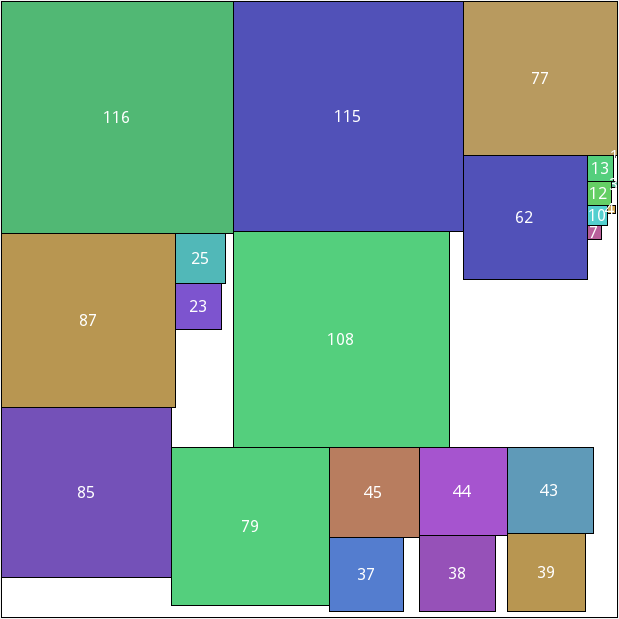
\includegraphics[width=0.4\textwidth]{squares}
  \caption{Beispiel für eine Visualisierung des Beladungsproblems}
\end{figure}

\subsubsection{Technische Voraussetzungen an die Teilnehmerprogramme}

Die Teilnehmerprogramme benötigen keine grafische Oberfläche und müssen auch
keine Netzwerkkommunikation unterstützen, es genügen einfache
Kommandozeilenanwendungen.
Diese bekommen alle benötigten Daten (die Parameter, die das
zu lösende Problem beschreiben) über die Standardeingabe, nachdem sie gestartet
wurden\footnote{Zwischen dem Programmaufruf und der Übergabe der Daten ist
genügend Zeit um beispielsweise einen Interpreter oder eine VM zu laden, damit
alle Teilnehmer die gleiche Zeit zur Verfügung haben. Unabhängig von der
Implementierungssprache.}.
Das Format ist hierbei frei wählbar und sollte so gewählt werden, dass es für
die Teilnehmer möglichst einfach zu parsen ist.
Es ist zu beachten, dass die Standardeingabe anschließend vom Framework
nicht geschlossen wird (es folgt kein \texttt{EOF}, Teilnehmerprogramme sollten
auch nicht auf ein solches warten).

Die Bearbeitungszeit läuft ab der Übergabe der Problemparameter.
In dieser Zeit können die Teilnehmerprogramme beliebig viele Vorschläge machen.
Pro Vorschlag ist genau eine Zeile auf die Standardausgabe zu schreiben (das
Format ist auch hier frei wählbar).
Alle Lösungsvorschläge werden zur Weiterverarbeitung an die
``Bewertungskomponente'' (siehe \ref{sec:validator}) gesendet.

\subsection{Was macht das Framework dabei?}

Das Framework steuert den grundlegenden Ablauf des Wettbewerbs.
Dies beinhaltet das Starten und sichere Beenden sowie die Kommunikation mit den
Teilnehmerprogrammen und den Komponenten (siehe \ref{sec:components}).

Jedem Teilnehmerprogramm kann für die Ausführung ein eigener PC zugewiesen
werden (siehe \ref{sec:configuration}), damit allen zur Lösung des
Problems dieselbe Rechenleistung zur Verfügung steht, obwohl sie gleichzeitig
laufen.
Der Aufbau des Clusters wird dabei ebenfalls vom Framework übernommen.

Jede Problemstellung kann über mehrere Runden gespielt werden.
Hierfür speichert das Framework für die aktuell ausgewählte Problemstellung
einen Zustand (siehe \ref{sec:configuration}).
Der Zustand ist dabei eine beliebige Zeichenkette, die durch die ins Framework
eingehängten Komponenten manipuliert werden kann.
So kann der Zustand durch anwenden einzelner Teilnehmerlösungen verändert
werden, um beispielsweise in der nächsten Runde das Problem mit einer leicht
veränderten Ausgangssituation zu Lösen.

Dieser Zustand könnte z.B. bei dem bereits erwähnten Beladungsproblem
verwendet werden. So könnte man als Zustand die Menge der zur Verfügung
stehenden Quadrate definieren. Jetzt lässt man eine Runde laufen und nimmt
dann die in der besten Lösung verwendeten Quadrate aus der Menge (modifizierter
Zustand). Damit ist diese Lösung in der nächsten Runde ausgeschlossen.

Eine andere interessante Verwendung des Zustandes wäre in einem Scrabble-%
basierten Problem möglich. Hier könnte man die Anfangsbelegung des Spielfelds
als Zustand nutzen und die beste Lösung jeweils der Belegung hinzufügen, so dass
sie ebenfalls in der nächsten Runde nicht wieder als gültige Lösung eingereicht
werden kann.

\subsection{Architektur}

\subsubsection{Überblick}

Um das Framework auf einen Wettbewerb anpassen zu können ist die Logik, die
abhängig von der konkreten Problemstellung ist, in externe Komponenten
ausgelagert. Diese Komponenten können in einer beliebigen Sprache
implementiert werden.
Die Kommunikation mit dem Framework erfolgt in JSON über die
Standard-Ein-/Ausgabe (siehe \ref{sec:components}).
Je nach konkreter Problemstellung können für einige Funktionen
Standardkomponenten verwendet werden, um Entwicklungsaufwand zu sparen.
Die Standard-Komponente für das ``user interface'' zum Beispiel ist sehr
allgemein gestaltet und sollte mit jeder Problemstellung funktionieren, sofern
keine Visualisierung gewünscht ist.

\begin{figure}[ht]
  \centering
  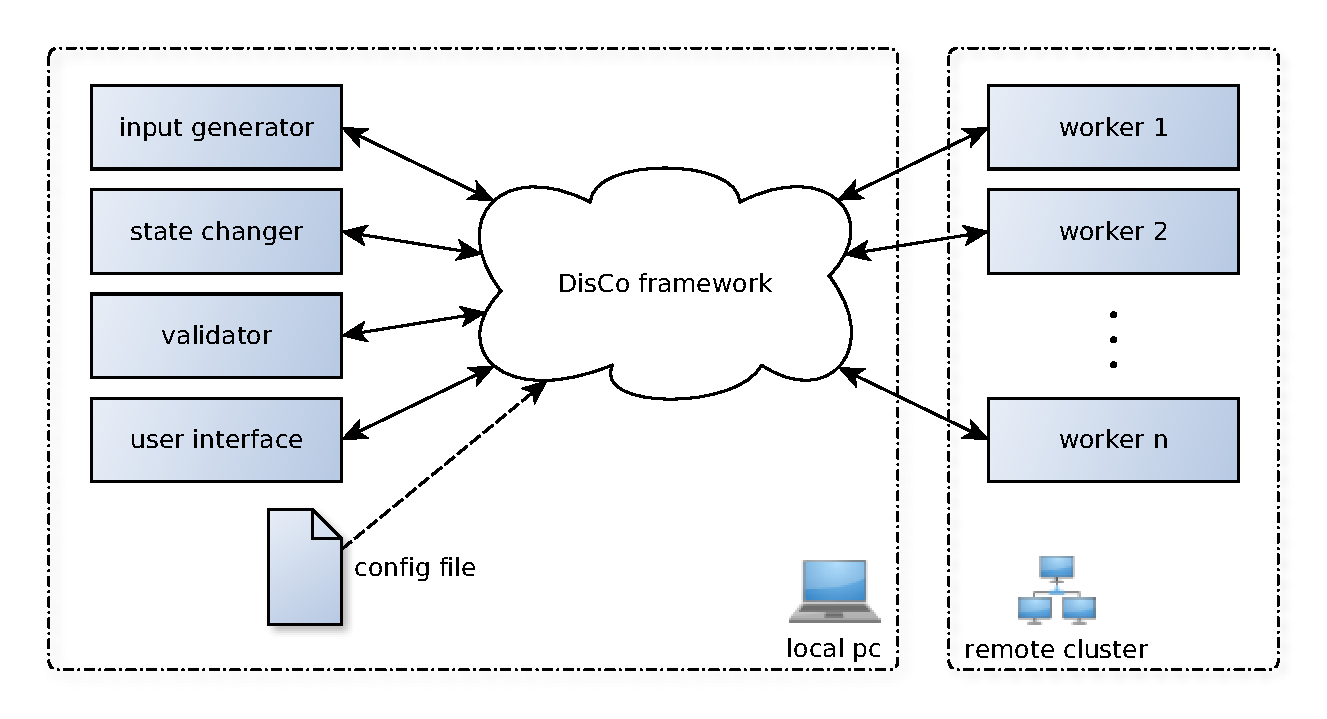
\includegraphics[width=\textwidth]{overview}
  \caption{Aufbau des Frameworks}
\end{figure}

\subsubsection{Komponenten}

Die genauen Protokolle, über die die Komponenten mit dem Framework
kommunizieren, sind unter \ref{sec:components} aufgeführt.

\begin{description}
  \item[input generator]
    Erzeugt die problembeschreibenden Daten, die alle Teilnehmerprogramme über
    die Standardeingabe bekommen.
    Für die Erzeugung dieser Daten bekommt der ``input generator'' die
    Problemspezifikation für das aktuell ausgewählte Problem sowie den aktuellen
    Zustand.
    Die Problemspezifikation und der Initialzustand können in der
    Konfigurationsdatei definiert werden.

    Im einfachsten Fall wird kein rundenübergreifender Zustand benötigt (wenn
    jedes Problem nur einmal gespielt werden soll) und die
    Problemspezifikationen in der Konfigurationsdatei können unverändert als
    Problembeschreibung an die Teilnehmerprogramme gesendet werden.

    Der ``input generator'' kann aber auch auf Basis der Problemspezifikation
    eine Zufallskomponente ins Spiel bringen. Im Fall eines Scrabble-Problems
    könnten z.B. ein Wörterbuch in der Problemspezifikation und
    die Belegung des Spielfelds als Initialzustand definiert werden.
    Die Auswahl der zur Verfügung stehenden Buchstaben erfolgt dann aber
    zufällig, z.B. basierend auf den im Wörterbuch vorkommenden Buchstaben.

  \item[state changer]
    Verändert den aktuellen Zustand des Problems durch Anwendung einer
    Teilnehmerlösung.
    Nicht jeder Wettbewerb benötigt einen Zustand (z.B. wenn die Probleme nicht
    über mehrere Runden gespielt werden sollen), in diesem Fall muss der ``state
    changer'' nicht ausgetauscht werden. Die Standardkomponente für den ``state
    changer'' gibt den Zustand einfach unverändert zurück.

    Ein Beispiel für einen Wettbewerb mit veränderbarem Zustand wäre das
    Beladungsproblem, wenn hier alle Quadrate, die in der Lösung eines
    bestimmten Teilnehmers verwendet wurden, aus der Liste der verfügbaren
    Quadrate für die nächste Runde entfernt werden sollen.

  \item[validator]
    Die Bewertungskomponente bekommt den von einem Teilnehmerprogramm
    abgegebenen Vor\-schlag (zusammen mit der zugehörigen Problembeschreibung)
    und überprüft diesen auf Gültigkeit und Qualität.
    Wird ein Vorschlag von der ``validator''-Komponente als ungültig erkannt,
    wird das Teilnehmerprogramm vom Framework deaktiviert.
    Andernfalls erhält es die vom ``validator'' bestimmte Punktzahl.
    Dabei liegt es im Ermessen des Implementierers, wann und ob überhaupt
    Vorschläge als ungültig erklärt werden sollen.

  \item[user interface]
    Ist für die Steuerung des Ablaufs (Auswahl eines Problems, starten/beenden
    einer Runde, ...) und die Darstellung zuständig.
    Üblicherweise stellt das ``user interface'' eine Tabelle dar, in der die
    Teilnehmer, ihre Punkte und der letzte Vorschlag angezeigt werden.

    Im Gegensatz zu den anderen Komponenten kann es mehrere (unterschiedliche)
    ``user interface''-Komponenten geben.
    Dies ist hilfreich für Problemstellungen bei denen die Visualisierung der
    Lösungen mehr Platz in Anspruch nimmt und beispielsweise auf einem separaten
    Monitor angezeigt werden soll.

    Außerdem kann so z.B. die Standardkomponenten für die Listenansicht
    verwendet werden und zusätzlich eine getrennte Komponente für die
    problemspezifische Visualisierung.
\end{description}

\subsection{Ablauf}

Die Durchführung eins Wettbewerbs mit dem Framework erfolgt nach folgendem
Ablauf:

\begin{enumerate}
  \item Starten des Frameworks
        \begin{itemize}
          \item[\(\rightarrow\)] Die Konfigurationsdatei wird gelesen.
          \item[\(\rightarrow\)] Die Komponenten werden gestartet.
          \item[\(\rightarrow\)] Das Rechner-Cluster wird aufgebaut und die
            Teilnehmerprogramme werden auf den entfernten Rechnern gestartet.
            Sie bekommen aber noch keine Problembeschreibung.
        \end{itemize}

  \item Auswahl einer Problemstellung über die Benutzeroberfläche.
        \begin{itemize}
          \item[\(\rightarrow\)] Der ``input generator'' erzeugt die
            Problembeschreibung für die Teilnehmerprogramme.
        \end{itemize}

  \item Starten einer Runde des ausgewählten Problems über die
        Benutzeroberfläche.
        \begin{itemize}
          \item[\(\rightarrow\)] Die Teilnehmerprogramme bekommen die
            Problembeschreibung und können Lösungsvorschläge einreichen.
        \end{itemize}

  \item Jeder eingereichte Lösungsvorschlag wird vom ``validator'' bewertet.
        \begin{itemize}
          \item[\(\rightarrow\)] In der Benutzeroberfläche wird der letzte
            Vorschlag (inkl. Bewertung) jedes Teilnehmers angezeigt.
        \end{itemize}

  \item Nach Ablauf der Rundenzeit werden alle Teilnehmerprogramme beendet und
    direkt ohne Input neugestartet, damit sie für die nächste Runde bereit sind.
    Das Framework wartet noch auf die Validierung eventuell in der Warteschlange
    vorhandener Vorschläge und erklärt dann die Runde für beendet.

  \item Über die Benutzeroberfläche kann nun
        \begin{itemize}
          \item ein anderes Problem ausgewählt werden (weiter bei Schritt 2.),
            oder
          \item eine weitere Runde mit dem aktuellen Problem gestartet werden
            (weiter bei Schritt 3.).
            In diesem Fall sollte der Zustand vorher verändert werden (durch
            Anwenden einer Teilnehmerlösung über die Benutzeroberfläche).
        \end{itemize}

\end{enumerate}


\section{Benutzung}

\subsection{Implementierung der Komponenten}
\label{sec:components}

Die vier Komponenten, die die wettbewerbsspezifische Logik implementieren,
werden beim Starten des Frameworks mitgestartet und laufen solange, bis das
Framework wieder beendet wird.
Sollte eine Komponente mal abstürzen, wird sie automatisch neugestartet.
Auf diese Weise stehen die Komponenten immer für Anfragen bereit.
Der Verzeichnis- und Dateiname der einzelnen Komponenten kann in der
Konfigurationsdatei (siehe \ref{sec:configuration}) eingestellt werden.
Die Kommunikation mit dem Framework erfolgt über die Standard-Ein/Ausgabe.

Beispielkomponenten finden Sie unter den in \ref{sec:configexample}
angegebenen Pfaden.

\subsubsection{Eingabeerzeuger (\texttt{input generator})}
Der ``input generator'' bekommt vor dem Start einer neuen Runde eine JSON
Nachricht mit folgenden Elementen:
\begin{componenttable}
  problem & string & die Problemspezifikation aus der Konfigurationsdatei\\
  state   & string & der aktuelle Zustand\\
\end{componenttable}
\begin{example}{Beispiel:}
{ "problem" : "[1,2,3,4]", "state" : "42" }
\end{example}

Die Antwort muss ebenfalls in JSON erfolgen und den folgenden Wert enthalten:
\begin{componenttable}
  worker input & [\,string\,] & Die Eingabe, die die Teilnehmerprogramme
                                anschließend als Problembeschreibung erhalten.
                                Die Strings dürfen keine Zeilenumbrüche
                                enthalten, da sie zeilenweise an die
                                Teilnehmerprogramme ausgegeben werden
                                (Ein Wert pro Zeile).\\
\end{componenttable}
\begin{example}{Beispiel:}
{ "worker input" : ["[1,2,3,4]", "42"] }
\end{example}

\subsubsection{Bewertungseinheit (\texttt{validator})}
\label{sec:validator}
Der ``validator'' ist für die Bewertung der Lösungsvorschläge zuständig.
Für jeden Vorschlag, den eines der Teilnehmerprogramme einreicht, bekommt der
``validator'' vom Framework eine JSON-Nachricht mit folgenden Elementen:
\begin{componenttable}
  input  & [\,string\,] & Beschreibung des Problems, die auch das
                          Teilnehmerprogramm bekommen hat.\\
  output & string       & Der eingereichte Lösungsvorschlag des
                          Teilnehmerprogramms.\\
\end{componenttable}
\begin{example}{Beispiel:}
{ "input" : ["[1,2,3]", "6"], "output" : "[(0,0,3)]" }
\end{example}

Die Antwort muss ebenfalls in JSON erfolgen und die folgenden Werte enthalten:
\begin{componenttable}
  score   & number & Qualität des Vorschlags.
                     Negative Werte stehen für eine ungültige Lösung.\\
  caption & string & Kurzer Beschreibungstext zur Anzeige in der grafischen
                     Oberfläche. Dies kann entweder direkt der Vorschlag
                     sein oder eine Umschreibung, mit der Menschen mehr
                     anfangen können, siehe Beispiel.\\
\end{componenttable}
\begin{example}{Beispiele:}
{ "score" : 9, "caption" : "25% coverage" }
{ "score" : -1, "caption" : "invalid solution ..." }
\end{example}

Die Kommunikation zwischen Framework und Komponente ist synchron, der
``validator'' bekommt also erst den nächsten Vorschlag, nachdem der aktuelle
validiert wurde.

Wird eine Lösung als ungültig bewertet (negative Punktzahl), so wird das
Teilnehmerprogramm vom Framework beendet und deaktiviert (dies kann über das
``user interface'' rückgängig gemacht werden).


\subsubsection{Zustandsveränderer (\texttt{state changer})}
Der ``state changer'' bekommt eine JSON
Nachricht mit folgenden Elementen:
\begin{componenttable}
  proposition & string & Die Lösung des ausgewählten Teilnehmerprogramms.\\
  state       & string & Der aktuelle Zustand.\\
\end{componenttable}
\begin{example}{Beispiel:}
{ "proposition" : "(1+2+3+4)", "state" : "200" }
\end{example}

Die Antwort muss ebenfalls in JSON erfolgen und den folgenden Wert enthalten:
\begin{componenttable}
  state & string & Der neue Zustand.\\
\end{componenttable}
\begin{example}{Beispiel:}
{ "state" : "210" }
\end{example}

Die Kommunikation zwischen Framework und Komponente ist synchron.


\subsubsection{Benutzeroberfläche (\texttt{user interface})}
Über die Benutzeroberfläche kann der Ablauf des Wettbewerbs gesteuert werden.
Dies geschieht über einfache JSON Nachrichten, die an das Framework gesendet
werden können:

\begin{description}
  \item\texttt{\{ "{}action": }\textit{Aktion}%
       \texttt{,\ }\textit{Parametername}%
       \texttt{:\ }\textit{Parametertyp}%
       \texttt{ \}}
\end{description}

Wobei folgende Aktionen möglich sind (der Parameter wird nicht bei allen
Aktionen benötigt):
\par\begin{description}\item

\newcommand{\noparam}{\multicolumn{2}{c}{--- \textit{ohne Parameter} ---}}

\begin{tabularx}{\linewidth}{>{\ttfamily}l >{\ttfamily}l >{\ttfamily}l X}
  \normalfont Aktion & \multicolumn{2}{c}{Parameter} & Beschreibung \\
  & \normalfont Name & \normalfont Typ & \\
  \hline
  block worker      & worker id   & string & blockiert den Teilnehmer mit der
                                             angegebenen \textit{worker id} \\
  unblock worker    & worker id   & string & reaktiviert den Teilnehmer mit der
                                             angegebenen \textit{worker id} \\
  choose problem    & problem idx & number & wählt das angegebene Problem aus \\
  start round       & \noparam             & startet die Runde, indem allen
                                             Teilnehmerprogrammen die Problem\-%
                                             beschreibung gesendet wird \\
  kill all workers  & \noparam             & beendet alle Teilnehmerprogramme
                                             sofort (sie werden anschließend
                                             neugestartet) und beendet damit
                                             auch die aktuelle Runde \\
  apply proposition & worker id   & string & übernimmt die Antwort des
                                             angegebenen Teilnehmerprogramms in
                                             den aktuellen Zustand \\
  save game state   & file path   & string & speichert den aktuellen Zustand des
                                             Wettbewerbs \\
  load game state   & file path   & string & lädt einen gespeicherten
                                             Wettbewerbszustand \\
  add scores        & \noparam             & addiert die Punkte der aktuellen
                                             Runde auf die Gesamtpunkte \\
  quit program      & \noparam             & beendet das gesamte Framework \\
  get all data      & \noparam             & Alle Daten erfragen: Workerinfos,
                                             Zustand, Problemliste, ... \\
\end{tabularx}
\end{description}

\begin{example}{Beispiele:}
{ "action" : "block worker", "worker id" : "pwb01" }
{ "action" : "choose problem", "problem idx" : 2 }
{ "action" : "start round" }
\end{example}

Nach jeder Änderung informiert das Framework die Benutzeroberflächen (es kann
mehrere geben) über die aktualisierten Daten mit Hilfe einer asynchronen JSON
Nachricht. Diese Nachrichten sind also im allgemeinen keine Antworten auf
die obenstehenden ``actions'', sondern können zu jedem Zeitpunkt getriggert
werden. Format der ``event''-Nachrichten:

\begin{description}
  \item\texttt{\{ "{}event": }\textit{Event}%
       \texttt{,\ }\textit{Parameter...}%
       \texttt{ \}}
\end{description}

Folgende \textit{Event}s sind dabei möglich (je nach Eventtyp sind weitere
Parameter vorhanden):

\begin{description}[\compact\breaklabel\setlabelstyle{\ttfamily}]
  \item[worker updated]
    Dieses Event wird gesendet wenn sich an den teilnehmerspezifischen Daten
    etwas geändert hat. Z.B. wenn ein Teilnehmerprogramm einen Lösungsvorschlag
    sendet oder wenn in der Benutzeroberfläche ein Teilnehmer geblockt/%
    reaktiviert wird. Die Daten werden in einer Liste mit genau acht Elementen
    und dem Namen \verb+"worker data"+ übertragen:
    \begin{enumerate}
      \item Die ID des Teilnehmers.
            \type{string}
      \item Der zuletzt gesendete Lösungsvorschlag des Teilnehmerprogramms, oder
            \texttt{null}, wenn noch keiner gesendet wurde.
            \type{string | null}
      \item Die vom ``validator'' bestimmte Kurzbeschreibung des
            Lösungsvorschlags.
            \type{string}
      \item Die vom ``validator'' bestimmte Punktzahl des
            Lösungsvorschlags.
            \type{number}
      \item Die normierte Punktzahl des Lösungsvorschlags.
            Diese wird erst nach dem Rundenende berechnet, da die Lösung des
            besten Teilnehmers als Maßstab genommen wird.
            \type{number}
      \item Die Summe der erreichten Punkte über mehrere Runden
            (für das aktuelle Problem).
            \type{number}
      \item Ob das Teilnehmerprogramm geblockt ist.
            Aktive Teilnehmer sind mit dem Wert \verb+"no"+ gekennzeichnet,
            ausgeschiedene Teilnehmer mit einem JSON Objekt welches angibt,
            als wievielter dieser deaktiviert wurde. Das ist entscheidend, wenn
            man den Gewinner im K.O.-Prinzip ermittelt.
            \type{string | \{ "{}idx": number \}}
      \item Ob das Teilnehmerprogramm gerade rechnet (\texttt{true}) oder nicht
            (\texttt{false}).
            \type{boolean}
    \end{enumerate}
    \begin{example}{Beispiele:}
{ "event": "worker updated",
  "worker data": ["pwb01", "((1 + 2) + (3 + 4))", "1+2+3+4",
                  200, 0, 2000, "no", true] }
{ "event": "worker updated",
  "worker data": ["pwb02", "foo", "Invalid syntax",
                  0, 0, 2000, {"idx": 0}, false] }
    \end{example}
    \vspace{-\baselineskip}

  \item[round started]
    Dieses Event wird ausgelöst, sobald eine Runde durch die Aktion
    \verb+"start round"+ (siehe oben) gestartet wird.
    Der Parameter \verb+"round number"+ (Typ: \verb+number+) gibt an, die
    wievielte Runde gestartet wurde.
    \begin{example}{Beispiel:}
{ "event": "round started", "round number": 1 }
    \end{example}
    \vspace{-\baselineskip}

  \item[round ended]
    Dieses Event wird ausgelöst, sobald die für dieses Problem eingestellte Zeit
    abgelaufen ist, alle Teilnehmerprogramme beendet wurden und auch alle
    Lösungsvorschläge bewertet wurden.
    Der Parameter \verb+"round number"+ (Typ: \verb+number+) gibt an, die
    wievielte Runde beendet wurde.
    \begin{example}{Beispiel:}
{ "event": "round ended", "round number": 1 }
    \end{example}
    \vspace{-\baselineskip}

  \item[worker input changed]
    Diese Nachricht wird gesendet, wenn sich durch die Auswahl eines anderen
    Problems oder durch Aktualisierung des Zustands die Problemspezifikation für
    die Teilnehmerprogramme ändert.
    Der Parameter \verb+"worker input"+ (Typ: \texttt{[\,string\,]} gibt dabei
    die neue Problembeschreibung an. Die Strings in der Liste sind die Zeilen,
    die auch die Teilnehmerprogramme beim Starten der Runde erhalten.
    \begin{example}{Beispiel:}
{ "event": "worker input changed",
  "worker input": ["[1,2,3,4]", "42"] }
    \end{example}
    \vspace{-\baselineskip}

  \item[save game state]
    Als Reaktion auf eine \verb+"save game state"+--Aktion gibt diese Nachricht
    mit einem Parameter \verb+"result"+ (Typ: \verb+"string"+) an, ob das
    Speichern erfolgreich war.
    Mögliche Rückgabewerte sind:
    \begin{description}[\compact\setlabelphantom{enotdir}\setlabelstyle{\ttfamily}]
      \item[ok]      Speichern der Datei war erfolgreich
      \item[eacces]  Berechtigungen fehlen
      \item[eisdir]  Unter diesem Namen existiert ein Verzeichnis
      \item[enoent]  Pfad existiert nicht
      \item[enospc]  Speicherplatz nicht ausreichend
      \item[enotdir] Pfad enthält Datei, wo Verzeichnis sein sollte
    \end{description}
    \begin{example}{Beispiel:}
{ "event": "save game state", "result": "ok" }
    \end{example}
    \vspace{-\baselineskip}

  \item[load game state]
    Als Reaktion auf eine \verb+"load game state"+--Aktion gibt diese Nachricht
    mit einem Parameter \verb+"result"+ (Typ: \verb+"string"+) an, ob das
    Laden erfolgreich war.
    Mögliche Rückgabewerte sind:
    \begin{description}[\compact\setlabelphantom{enotdir}\setlabelstyle{\ttfamily}]
      \item[ok]      Laden der Datei war erfolgreich
      \item[eacces]  Berechtigungen fehlen
      \item[eformat] Dateiinhalt hat das falsche Format
      \item[eisdir]  Unter diesem Namen existiert ein Verzeichnis
      \item[enoent]  Pfad existiert nicht
      \item[enotdir] Pfad enthält Datei, wo Verzeichnis sein sollte
    \end{description}
    \begin{example}{Beispiel:}
{ "event": "load game state", "result": "ok" }
    \end{example}
    \vspace{-\baselineskip}

  \item[problem chosen]
    Dieses Event wird ausgelöst, wenn durch die Aktion \verb+"choose problem"+
    (siehe oben) eine andere Problemstellung ausgewählt wurde. Der Parameter
    \verb+"problem idx"+ (Typ: \verb+number+) gibt dabei den Index des
    ausgewählten Problems an. Mit diesem kann aus der Nachricht
    \verb+"all data"+ (siehe unten) die genaue Problembeschreibung ermittelt
    werden.
    \begin{example}{Beispiel:}
{ "event": "problem chosen", "problem idx": 2 }
    \end{example}
    \vspace{-\baselineskip}

  \item[problem state changed]
    Wird ein Problem über mehrere Runden gespielt, liefert diese Nachricht mit
    dem Parameter \verb+"problem state"+ den aktuellen Zustand, sobald sich
    dieser durch die Aktion \verb+"apply proposition"+ (siehe oben) ändert.
    \begin{example}{Beispiel:}
{ "event": "problem state changed",
  "problem state": "neue Zustand"}
    \end{example}
    \vspace{-\baselineskip}

  \item[all data]
    Dieses Event wird automatisch nach dem Start der Benutzeroberfläche gesendet
    oder wenn mit der Aktion \verb+"get all data"+ danach gefragt wird.
    Es enthält folgende Elemente:
    \begin{description}[\compact\setlabelstyle{\ttfamily}]
      \item[running]
        gibt an, ob aktuell eine Runde läuft
        \type{boolean}
      \item[workers]
        Liste aller Teilnehmer und ihrer Daten.
        \type{[\,TeilnehmerDaten\,]}
        Die \verb+TeilnehmerDaten+ werden jeweils in einer Liste mit genau neun
        Elementen angegeben (ähnlich wie im \verb+"worker updated"+--Event):
        \begin{enumerate}
          \item Die ID des Teilnehmers.
                \type{string}
          \item Der Name des Teilnehmerprogramms.
                \type{string}
          \item Die Gruppe, in der der Teilnehmer antritt (laut
                Konfigurationsdatei, siehe \ref{sec:configuration}).
                \type{string}
          \item[4.--10.] genau wie die Punkte 2.--8. im
                \verb+"worker updated"+--Event (siehe oben):\\
                letzter Vorschlag, Kurzbeschreibung, Punktzahl, normierte
                Punktzahl, Punktsumme, der geblockt-Status und ob das
                Teilnehmerprogramm gerade rechnet.
        \end{enumerate}
      \item[problems]
        Liste der Problemstellungen und ihrer Daten.
        \type{[\,ProblemDaten\,]}
        Die \verb+ProblemDaten+ werden jeweils in einer Liste mit genau fünf
        Elementen angegeben:
        \begin{enumerate}
          \item Der Index der Problemstellung, so wie er auch in der Aktion
                \verb+"choose problem"+ und im Event \verb+"problem chosen"+
                verwendet wird.
                \type{number}
          \item Die Kurzbeschreibung des Problems aus der Konfigurationsdatei.
                \type{string}
          \item Die Spezifikation des Problems aus der Konfigurationsdatei,
                die auch der ``input generator'' bekommt.
                \type{string}
          \item Die für eine Runde zur Verfügung stehende Zeit in Millisekunden.
                \type{number}
          \item Der Initialzustand des Problems aus der Konfigurationsdatei.
                \type{string}
        \end{enumerate}
      \item[problem idx]
        Der Index des aktuell ausgewählten Problems.
        \type{number}
      \item[round]
        Die Nummer der aktuell laufenden Runde bzw. der zuletzt beendeten Runde,
        je nachdem, ob gerade eine Runde läuft (siehe \verb+running+).
        \type{number}
      \item[worker input]
        Die Definition des ausgewählten bzw. laufenden Problems, so, wie sie
        auch die Teilnehmerprogramme bekommen werden bzw. haben.
        \type{[~string~]}
      \item[state]
        Der Zustand des aktuellen Problems.
        \type{string}
    \end{description}
    \begin{example}{Beispiel:}
{ "event": "all data",
  "running": false,
  "workers": [
    ["pwb01", "hello", "", "2 + 4", "2+4", 6, 0, 0, "no", false],
    ["pwb02", "foo",   "", null,    "",    0, 0, 0, "no", false],
    ["pwb03", "blub",  "", "3 + 3", "3+3", 9, 0, 0, "no", false]
  ],
  "problems": [ [0, "erstes Problem", "[1,2,3,4]", 5000, "42"],
                [1, "zweites Problem", "[2,3,4]", 2000, "42"] ],
  "problem idx": 1,
  "round": 1,
  "worker input": ["[1,2,3,4]", "42"],
  "state": "Zustand" }
    \end{example}
    \vspace{-\baselineskip}

\end{description}

\subsection{Vorbedingungen}

Damit das Framework richtig funktioniert, müssen ein paar Voraussetzungen
erfüllt sein.

\subsubsection{Zugriff per SSH}

Der Aufbau des Rechner-Clusters, auf dem die Teilnehmerprogramme ausgeführt
werden, erfolgt per SSH.
Hierfür ist es erforderlich, dass ein Login auf den betroffenen Rechnern ohne
Angabe von Benutzername oder Passwort erfolgen kann.
Dies lässt sich über eine Public-Key-Authentifizierung erreichen.
Ist der Benutzername auf den entfernten Rechnern nicht derselbe wie lokal,
kann dieser in der eigenen SSH-Konfiguration
(\texttt{\(\sim\)/.ssh/config})
angegeben werden:
\begin{example}{}
Host 192.168.1.*
     User discoUser
\end{example}

Binärdateien des Frameworks und Teilnehmerprogramme müssen auf allen
Rechnern dem per SSH eingeloggten Nutzer unter dem selben, konfigurierbaren
Pfad zur Verfügung stehen.

Befinden sich diese Daten auf einem Benutzerprofil, das erst beim Login von
einem Server geladen wird, so muss sichergestellt werden, dass dies vor dem
Starten des Framworks passiert (z.B. indem manuell eine SSH-Verbindung mit
den betroffenen Profilen aufgebaut wird).

Das Framework kann auch vollständig auf dem lokalen Rechner ausgeführt werden.
Dies ist jedoch nur zu Testzwecken sinnvoll, da dann alle Teilnehmerprogramme
gleichzeitig und zusätzlich zum Framework auf dem lokalen Rechner laufen.
Allerdings wird so kein SSH und damit auch keine
Public-Key-Authentifizierung benötigt.
Erreicht werden kann dies, indem alle IP-Adressen des Clusters in der
Konfigurationsdatei auf den Wert des Makros ``\texttt{LOCAL\_IP}'' des
\texttt{Makefile}s (``\texttt{127.0.0.1}'') gesetzt werden.

\subsubsection{Benötigte Pakete}

Auf dem Steuerungsrechner, auf dem das Framework und die externen Komponenten
laufen, werden folgende Pakete benötigt:
\begin{itemize}
  \item \texttt{erlang} R16B oder 17\\
        Für die Programme \texttt{erl} und \texttt{escript}.\\
        Die Kompatibilität zu anderen Versionen ist nicht ausgeschlossen,
        allerdings wurde das Framework nur mit den Versionen R16B und 17
        getestet.
        Bei abweichenden Versionen muss ggf. der Wert von
        \texttt{require\_otp\_vsn} in der Datei \texttt{rebar.config}
        angepasst werden.
  \item \texttt{make}\\
        Ist nicht zwingend erforderlich, erlaubt aber die Nutzung des Makefiles
        zum Erzeugen und Starten des Frameworks.
        Viele Aktionen werden an \texttt{rebar} (ein Buildtool für Erlang)
        weitergeleitet.
  \item \texttt{git}\\
        Das Buildtool \texttt{rebar} verwendet \texttt{git} um die verwendeten
        Erlang-Bibliotheken herunterzuladen (siehe auch \texttt{rebar.config}).
  \item ssh client (z.B. \texttt{openssh})\\
        Wird benötigt, um das entfernte Cluster aufzubauen.\\
        Falls das Framework komplett auf dem lokalen Rechner ausgeführt werden
        soll, wird kein SSH benötigt.
  \item \texttt{ip} (optional)\\
        Zur automatischen Ermittlung der eigenen externen IP-Adresse für den
        Makro-Wert ``\texttt{LOCAL\_IP}'' im \texttt{Makefile}.
  \item \texttt{rsync} (optional)\\
        Wird nur beim optionalen Aufruf von ``\texttt{make distribute}'' für die
        Verteilung des Erlang-Codes auf die entfernten Cluster-Rechner benötigt.
  \item Pakete, die von den verwendeten Komponenten zur Ausführung benötigt
        werden. Die wettbewerbsunabhängige Benutzeroberfläche benötigt
        \texttt{python} und \texttt{pyqt4-dev-tools}.
\end{itemize}

Auf den Rechnern des Clusters, auf denen die Teilnehmerprogramme laufen sollen,
werden folgende Pakete benötigt:
\begin{itemize}
  \item Pakete, die evtl.\ von den Teilnehmerprogrammen zur Ausführung benötigt
    werden
  \item \texttt{erlang} (gleiche Version wie auf dem Steuerungsrechner)
  \item \texttt{rsync} (wie Steuerungsrechner)
  \item ssh server (wie Steuerungsrechner)
\end{itemize}


\subsection{Konfiguration}
\label{sec:configuration}

Die Einstellungen, die für einen Wettbewerb benötigt werden, können
in einer Konfigurationsdatei angegeben werden.
Dies sind unter anderem die Pfade zu den Komponenten, die die
wettbewerbsspezifische Logik implementieren, die Liste der IP-Adressen
des Clusters, auf dem die Teilnehmerprogramme ausgeführt werden sollen
und die zu spielenden Problemstellungen.

Welche Konfigurationsdatei zu verwenden ist, wird direkt im \texttt{Makefile}
definiert.

\subsubsection{Syntax}
Die Konfiguration erfolg in Erlang-Syntax und besteht aus einer Liste, in der
für jede Erlang-OTP-Application (in diesem Fall nur eine: ``disco'') eine
Liste von Schlüssel-Wert-Paaren in Form von Tupeln definiert wird (siehe auch:
\url{http://www.erlang.org/doc/man/config.html}).
\begin{lstlisting}
[
  {disco,
    [
      {key1, "value1"},
      {key2, 1337},
      {key3, ["hello", "world"]},
      {key4, {foo, 1, "2", []}},
    ]
  }
].
\end{lstlisting}
Hierbei ist der Schlüssel ein Atom und der Wert kann ein beliebiger Term
sein.
Welche Einstellungen es gibt und welche Werte dort erlaubt sind, wird anhand der
folgenden Beispielkonfiguration erläutert.

\subsubsection{Beispielkonfiguration}
\label{sec:configexample}

Den Quelltext der einzelnen Komponenten finden Sie an den unter
``local components'' angegebenen Pfaden.

\begin{lstlisting}
[
  {disco,
    [
      %% --- local components ---
      %% commands relative to the current directory:
      %% (barkeeper is the "input generator" and changer the "state changer")
      {validator, "make run -sC priv/countdown/components/validator/"},
      {barkeeper, "priv/general/components/barkeeper/barkeeper.rb"},
      {changer,   "priv/general/components/changer/changer.rb"},
      {gui,      ["make run -sC priv/general/components/gui/"]},

      %% --- remote workers ---
      %% remote directory containing the 'ebin', 'deps' and 'apps' folder
      %% If this is an empty string (default), the folder structure and
      %% location is assumed to be the same on master and slave nodes.
      {remote_node_path_prefix, "/home/stud/inf/inf9404/pwb/"},

      %% worker commands relative to the remote_node_path_prefix
      %% '%id%' will be replaced by the woker id (e.g. 'pwb_01'; see workers)
      {worker_run_cmd,  "make run  -sC priv/countdown/workers/%id%/"},
      {worker_name_cmd, "make name -sC priv/countdown/workers/%id%/"},
      {workers, [% {<worker id>, <ip address>, <additional information>}
                 {pwb01, '192.168.1.101', "students"},
                 {pwb02, '192.168.1.102', "students"},
                 {pwb03, '192.168.1.103', "students"},
                 {pwb04, '192.168.1.104', "alumni"},
                 {pwb05, '192.168.1.105', "alumni"},
                 {pwb06, '192.168.1.106', "staff"},
                 {pwb07, '192.168.1.107', "staff"}
                ]
      },

      %% When the cluster is started in parallel, multiple nodes are booted
      %% at the same time. The degree of parallelism can be adjusted through
      %% the slice size which determines the number of concurrent threads
      %% to use. Make sure `MaxStartups' in the config of your ssh daemon is
      %% large enough.
      {cluster_start_mode, parallel},  % :: sequential | parallel
                                       %                   (default: sequential)
      {startup_slice_size, 10},        % :: pos_integer()  (default: 10)

      %% Score calculation mode.
      %% raw:        the solution scores are added up
      %% normalized: the rounded percentage that this score has of the maximum
      %%             percentage from the current round is added up.
      %%             Example:
      %%             The worker A has 20 points. The best worker in the
      %%             current round, B, has 50 points. So worker A gets
      %%             40 normalized points added to his total score while
      %%             worker B gets 100 normalized points added.
      %% ranked:     The ``reverse rank'' gets added to the total score.
      %%             So when there are 12 workers, the worker with the
      %%             best solution gets 12 points, the one with the worst
      %%             solution gets just 1 point. In the case of multiple
      %%             solutions with equal scores, those workers share a
      %%             rank. So if all workers have equally good solutions,
      %%             all workers get 12 points added to their total score.
      {score_mode, ranked},            % :: raw | normalized | ranked
                                       % default: ranked

      %% --- list of problems to solve ---
      %% Each problem specification can be used for an arbitrary number of
      %% rounds.
      {problems, [%{<description>, <specification>, <answer time>, <state>}
                  {"First problem", "[1,1,2,3,5,8] 42",      1000, ""     },
                  {"Prime numbers", "[2,3,5,7,11,13,17] 42", 9000, ""     },
                  {"Impossible",    "nothing",                  0, ""     }
                 ]
      }
    ]
  }
].
\end{lstlisting}

\end{document}
